\documentclass[addpoints]{exam}

\usepackage{amsmath}
\usepackage{amssymb}
\usepackage{enumitem}
\usepackage{graphicx}
\usepackage{hyperref}
\usepackage{multicol}
\usepackage{tikz}
\usepackage{titling}
\usepackage{tabularx}


% Header and footer.
\pagestyle{headandfoot}
\runningheadrule
\runningfootrule
\runningheader{CS 113 Spring 201}{HW 4: Functions, Induction, Graphs}{\theauthor}
\runningfooter{}{Page \thepage\ of \numpages}{}
\firstpageheader{}{}{}

\boxedpoints
\printanswers

\newcommand\union\cup
\newcommand\interx\cap

\graphicspath{{images/}}

\title{Homework 4: Functions, Induction, Graphs}
\author{isomorphic-predicate}  % replace with your team name
\date{CS/MATH 113 Discrete Mathematics\\Habib University, Spring 2022}

\begin{document}
\maketitle

\begin{questions}

  \section*{Functions}
  
\question[5] Consider these functions from the set of students in a discrete mathematics class. Under what conditions is the
  function one-to-one if it assigns to every student,
  
  \begin{enumerate}[label=\alph*)]
  \item their mobile phone number.
    \begin{solution}
      let there be no two students with a common mobile phone number, 
      \newline Then only, the function that assigns to a student his or her mobile phone number is one-to-one.
    \end{solution}
  \item their student identification number.
    \begin{solution}
      Since there is a unique student ID number for everyone, no two students will be there 
      \newline such that they will have the same ID numbers. Therefore, the function that assigns
      \newline to a student, his or her, ID number is one-to=one. 
    \end{solution}
  \item their final grade in the class.
    \begin{solution}
      Since more than one student can have the same or similar final grade in the class, so the function will not be a one-to-one
      \newline generally. 
      \newline However, for it to be a one-to-one function, the number of students should be less or equal to 
      \newline to the number of final grades, and that all the students have different, unique, and disjoint grades. 
      \newline Then only it can be a one-to-one function. 
    \end{solution}
  \item their home town.
    \begin{solution}
      The function, generally, is not a one-to-one function because more than one student can have a similar
      \newline or same home town.
      \newline However, for it to be a one-to-one function, different students should have different, unique, and disjoint home towns.
    \end{solution}
  \item their Ehsas hour appointment.
    \begin{solution}
      Assuming that EHSAS hour appointments could be done at the same time, for the same TA, by multiple students,
      \newline It will not be a one-to-one function generally.
      \newline However, for it to be a one-to-one function, there should be a condition that only one student can book the appointment for a 
      \newline particular TA at a particular time. And that (all) different students have EHSAS appointments at different times with different TA's. 
      \newline This will thus, make it a one-to-one function.
    \end{solution}
  \end{enumerate}


\question[5] If $f$ and $f \circ g$ are one-to-one, does it follow that $g$ is one-to-one? Justify your answer.
  \begin{solution}
    We should note that $f$ is \textit{one-to-one} if and only if $\forall a, b \in x$ for $f(x)$, $f(a) = f(b) \implies a=b $ 
    \newline The function is \textit{onto} if and only if $\forall b \in B, \exists a \in A$, such that $f(a)=b$
    \newline Compositions of $f$ and $g$: $(f \circ g)(a) = f(g(a))$
    \newline
    \newline Given that $g: A \rightarrow B$ and,
    \newline Given that $f: B \rightarrow C$ and,
    \newline $f \circ g$ are one-to-one,
    \newline 
    \newline Lets assume $g(a) = g(b)$
    \newline Taking the function $f$ on each side:
    \newline $f(g(a)) = f(g(b))$
    \newline Using the definition of composition, we get that,
    \newline $(f \circ g)(a) = (f \circ g)(b)$
    \newline Since $(f \circ g)$ is one-to-one, $a=b$
    \newline 
    \newline Hence, $g(a) = g(b) \implies a=b$. Therefore, by definition of one-to-one functions, $g$ is one-to-one function is proved!
  \end{solution}

\question[5] Prove that a strictly decreasing function from $\mathbb{R}$ to itself is one-to-one. Give an example of a decreasing function from $\mathbb{R}$ to itself that is not one-to-one.
  \begin{solution}
    We should note that $f$ is \textit{one-to-one} if and only if $\forall a, b \in x$ for $f(x)$, $f(a) = f(b) \implies a=b $ 
    \newline $f$ is \textit{strictly increasing} if $x < y$, then $f(x) < f(y)$
    \newline $f$ is \textit{increasing} if $x < y$, then $f(x) \leq f(y)$
    \newline We should also note that a \textit{ceiling function} is $\lceil x \rceil$: smallest integer that is greater than or equal to $x$.
    \newline
    \newline Given that $f: R \mapsto R$ is a strictly decreasing function,
    \newline $f$ is a strictly decreasing function implies: if $x < y$, then $f(x) > f(y)$
    \newline We assume that $f(a) = f(b)$ that leads us To
    \newline if $a < b$ then it's an increasing function where $f(a) > f(b)$.
    \newline Therefore, it is not possible that $a < b$ when $f(a) = f(b)$
    \newline 
    \newline If $a > b$, then it's a strictly decreasing function where $f(b) > f(a).$
    \newline Here too, it is not possible that $b<a$ when $f(a) = f(b)$
    \newline
    \newline Because both conditions, $a>b$ and $a<b$ are not true, 
    \newline $a$ and $b$ should be the same, i.e., $a=b$
    \newline By definition of a one-to-one function, we needed to show that $a=b$ that we did,
    \newline Therefore, $f$ is a one-to-one function.
    \newline
    \newline $f(x) = \lceil x \rceil$ is an increasing function.
    \newline However, it is not a one-to-one function because it not possible for values to have the same image.
    \newline e.g. $f(2) = \lceil 2 \rceil = 2$
    \newline f(1.5) = $\lceil 1.5 \rceil = 2$
    \newline 
    \newline We take the function $g(x) = - \lceil x \rceil$, which is a decreasing function because of the negative sign.
    \newline This function is not a one-to-one function as some values have the same image.
    \newline e.g. $g(1) = - \lceil 1.5 \rceil = -2 $
    \newline $g(2.5) = - \lceil 2.5 \rceil = -2$

  \end{solution}
  
  \section*{Graphs}

\thispagestyle{empty}
\usetikzlibrary{fit,shapes}
\question To lift the spirits of the students on their return, Habib University has decided to build 4 new courtyards--Nature, Ice, Light, and Darkness. Designs are invited and bids are received for the courtyards from 4 architect firms as follows. Parveen Prime can design Nature, Light, and Darkness; Queen Quratulain can design Ice and Light; Reena Rani can design Light and Darkness; and Super Sonam can design Nature and Ice.
  \begin{parts}
  \part[5] Use a bipartite graph to model the four architects and the courtyards that they can design.
    % \begin{solution}
    %   Let the letters in nodes represent the certain architects and the courtyards.
    %   Where \textbf{N} is for \textit{Nature},
    %   \newline \textbf{I} is for \textit{Ice},
    %   \newline \textbf{L} if for \textit{Light},
    %   \newline and \textbf{D} is for Darkness courtyards respectively.
    %   \newline
    %   \newline Where \textbf{P} is for \textit{Parveen Prime},
    %   \newline \textbf{Q} is for \textit{Queen Quratulain},
    %   \newline \textbf{R} is for \textit{Reena Rani},
    %   \newline and \textbf{S} is for \textit{Super Sonam} firm respectively. 
    %   \newline
    %   \begin{tikzpicture}[main/.style = {draw, circle}] 
    %     \node[main] (2) [below of =1] {$Q$};
    %     \node[main] (4) [below of =3] {$S$};
    %     \node[main] (3) [below of =2] {$R$}; 
    %     \node[main] (1) {$P$}; 
    %     \node[main] (5) [above right of=1] {$D$}; 
    %     \node[main] (6) [below right of=5] {$I$};
    %     \node[main] (7) [below of=6] {$L$};
    %     \node[main] (8) [below of=7] {$N$};

    %     \draw (1) -- (5)
    %     \draw {1} -- (7)
    %     \draw (1) -- (8)
    %     \draw (2) -- (6)
    %     \draw (2) -- (7)
    %     \draw (3) -- (7)
    %     \draw (4) -- (6)
    %     \draw (4) -- (8)
    %     \draw (3) -- (5)

    %   \end{tikzpicture} 
    %\end{solution}
    \begin{solution}
        Let the letters in nodes represent the certain architects and the courtyards.
        Where \textbf{N} is for \textit{Nature},
        \newline \textbf{I} is for \textit{Ice},
        \newline \textbf{L} if for \textit{Light},
        \newline and \textbf{D} is for Darkness courtyards respectively.
        \newline
        \newline Where \textbf{P} is for \textit{Parveen Prime},
        \newline \textbf{Q} is for \textit{Queen Quratulain},
        \newline \textbf{R} is for \textit{Reena Rani},
        \newline and \textbf{S} is for \textit{Super Sonam} firm respectively. 
        \newline

      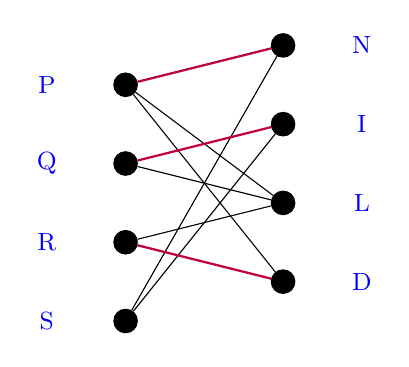
\begin{tikzpicture}
        \tikzstyle{node} = [draw,circle,fill=black,inner sep=3pt]
        \foreach \l/\x/\y in {a/0/0/, b/0/-1/, c/0/-2/, d/0/-3,
          e/2/0.5, f/2/-0.5, g/2/-1.5, h/2/-2.5 } {
          \node[node] (\l) at (\x,\y) {};
        }
  
        \foreach \a/\b in {a/e, a/g, a/h, b/f, b/g, c/g,c/h, d/e, d/f} {
          \draw (\a) -- (\b);
        }
        \foreach \a/\b in {a/P, b/Q, c/R, d/S} {
          \node[left of = \a]{\small\color{blue}\b};
        }
        \foreach \a/\b in {e/N, f/I, g/L, h/D} {
          \node[right of = \a]{\small\color{blue}\b};
        }
  
       \draw[purple,thick] (a) -- (e);
       \draw[purple,thick] (b) -- (f);
       \draw[purple,thick] (c) -- (h);
       %\draw[purple,thick] (d) -- (g);
       %Credits to Ahad Ali for helping me out in making the graph on LaTeX
      \end{tikzpicture}
    \end{solution}
    
  \part[5] Use Hall’s theorem to determine whether there is an assignment of architects to courtyards so that each architect is assigned one courtyard to design.
    \begin{solution}
      \begin{tabularx}{\textwidth}{X|X|X|X}
        $A$ & $N(A)$ & $|A|$ & $|N(A)|$ \\\hline\hline
        $\{\}$ & $\{\}$ & $0$ & $0$ \\
        $\{ P\}$  & $\{ D, L, N\}$ & $1$ & $3$ \\
        $\{ Q\}$ & $\{ I, L\}$ & $1$ & $2$ \\
        $\{ R\}$ & $\{ D, L\}$ & $1$ & $2$ \\
        $\{ S\}$ & $\{ I, N\}$ & $1$ & $2$ \\
        $\{ P,Q\}$ & $\{ D, I, L, N\}$ & $2$ & $4$ \\
        $\{ P, S\}$ & $\{ D, I, L, N\}$ & $2$ & $4$ \\
        $\{ R, S\}$ & $\{ D, I, L, N\}$ & $2$ & $4$ \\
        $\{ P, R\}$ & $\{ D, L, N\}$ & $2$ & $3$ \\
        $\{ Q, R\}$ & $\{ D, I, L\}$ & $2$ & $3$ \\
        $\{ Q, S\}$ & $\{ I, L, N\}$ & $2$ & $3$ \\
        $\{ P, Q, R\}$ & $\{ D, I, L, N\}$ & $3$ & $4$ \\
        $\{ P, Q, S\}$ & $\{ D, I, L, N\}$ & $3$ & $4$ \\
        $\{ P, R, S\}$ & $\{ D, I, L, N\}$ & $3$ & $4$ \\
        $\{ Q, R, S\}$ & $\{D, I, L, N\}$ & $3$ & $4$ \\
        $\{ P, Q, R, S\}$ & $\{ D, I, L, N\}$ & $4$ & $4$ \\
      \end{tabularx}
      Therefore, for all subsets of $A$ of $V_{1}$, $|A(N)| \geq |A|$, where $V_{1}$ are the vertices of architects
      \newline As a result, according to Hall's Theorem, from $V_{1}$ to $V_{2}$, there exists a complete matching, where $V_{2}$ are the vertices of names of courtyards.
    \end{solution}

  \part[5] Provide the assignment, if it exists, of architects to courtyards such that each architect is assigned to a courtyard that she can design.
    \begin{solution}
      Please note that the meaning of the alphabets is the same as that before in part (a)
      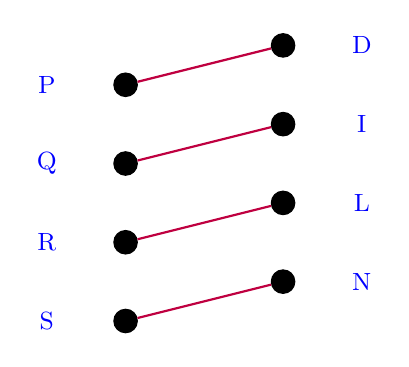
\begin{tikzpicture}
        \tikzstyle{node} = [draw,circle,fill=black,inner sep=3pt]
        \foreach \l/\x/\y in {a/0/0/, b/0/-1/, c/0/-2/, d/0/-3,
          e/2/0.5, f/2/-0.5, g/2/-1.5, h/2/-2.5 } {
          \node[node] (\l) at (\x,\y) {};
        }
  
        % \foreach \a/\b in {a/e, a/g, a/h, b/f, b/g, c/g,c/h, d/e, d/f} {
        %   \draw (\a) -- (\b);
        % }
        \foreach \a/\b in {a/P, b/Q, c/R, d/S} {
          \node[left of = \a]{\small\color{blue}\b};
        }
        \foreach \a/\b in {e/D, f/I, g/L, h/N} {
          \node[right of = \a]{\small\color{blue}\b};
        }
  
       \draw[purple,thick] (a) -- (e);
       \draw[purple,thick] (b) -- (f);
       \draw[purple,thick] (c) -- (g);
       \draw[purple,thick] (d) -- (h);
       %Credits to Ahad Ali for helping me out in making the graph on LaTeX
      \end{tikzpicture}
    \end{solution}
  \end{parts}
  
\question  The simple graphs $G_1 = (V_1,E_1)$ and $G_2 = (V_2,E_2$) are \textit{isomorphic} if there exists a one-to-one and onto function $f$ from $V_1$ to $V_2$ with the property that $a$ and $b$ are adjacent in $G_1$ if and only if $f(a)$ and $f(b)$ are adjacent in $G_2$, for all $a$ and $b$ in $V_1$. Such a function $f$ is called an \textit{isomorphism}. Two simple graphs that are not isomorphic are called \textit{non-isomorphic}.

  In other words, when two simple graphs are isomorphic, there is a one-to-one correspondence between the vertices of the two graphs that preserves the adjacency relationship. Isomorphism of simple graphs is an equivalence relation.

  Determine which of the following pairs of graphs are isomorphic. For each pair of graphs, provide an isomorphism (a bijection between the vertices of the graphs) or a rigorous argument that no such bijection exists.

  \begin{tabular}{cccc}
    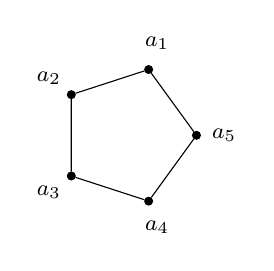
\begin{tikzpicture}
      \tikzstyle{node} = [draw,circle,fill=black,inner sep=1pt]
      \foreach \a in {1,2,...,5}{
        \draw (\a*360/5: 25pt) node(\a)[node]{};
        \draw (\a*360/5: 35pt) node{\footnotesize $a_\a$};
      }
      \path[draw] (1) -- (2) -- (3) -- (4) -- (5) -- (1);
    \end{tikzpicture}
    &
      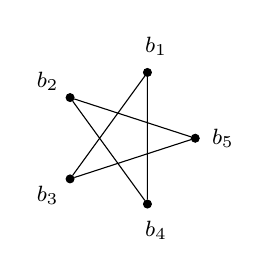
\begin{tikzpicture}
        \tikzstyle{node} = [draw,circle,fill=black,inner sep=1pt]
        \foreach \a in {1,2,...,5}{
          \draw (\a*360/5: 25pt) node(\a)[node]{};
          \draw (\a*360/5: 35pt) node{\footnotesize $b_\a$};
        }
        \path[draw] (2) -- (5) -- (3) -- (1) -- (4) -- (2);
      \end{tikzpicture}
    &
      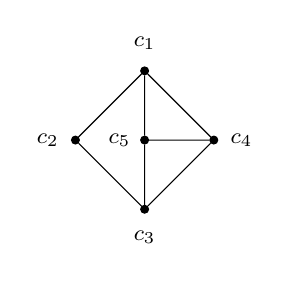
\begin{tikzpicture}
        \tikzstyle{node} = [draw,circle,fill=black,inner sep=1pt]
        \foreach \a in {1,2,...,4}{
          \draw (\a*360/4: 25pt) node(\a)[node]{};
          \draw (\a*360/4: 35pt) node{\footnotesize $c_\a$};
        }
        \node [node, label = left:\footnotesize $c_5$] (5) at (0,0) {};
        \path[draw] (1) -- (2) -- (3) -- (4) -- (1) -- (5) -- (4) -- (3) -- (5);
      \end{tikzpicture}
    &
      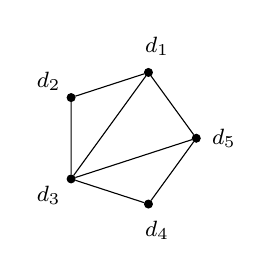
\begin{tikzpicture}
        \tikzstyle{node} = [draw,circle,fill=black,inner sep=1pt]
        \foreach \a in {1,2,...,5}{
          \draw (\a*360/5: 25pt) node(\a)[node]{};
          \draw (\a*360/5: 35pt) node{\footnotesize $d_\a$};
        }
        \path[draw] (1) -- (2) -- (3) -- (4) -- (5) -- (1) -- (3) -- (5);
      \end{tikzpicture}\\
    Graph A & Graph B & Graph C & Graph D    
  \end{tabular}    

  \begin{parts}
  \part[5] Graph A and Graph B
    \begin{solution}
      They are isomorphic since:
      $a_{2} \mapsto b_{2}, a_{1} \mapsto b_{5}, a_{5} \mapsto b_{3}$
      $a_{4} \mapsto b_{1}, a_{3} \mapsto 4$
    \end{solution}

  \part[5] Graph A and Graph C
    \begin{solution}
      %12345
      Graph A degree sequence: 2, 2, 2, 2, 2.
      \newline Graph C degree sequence: 3, 2, 3, 3, 3.
      \newline Since the degree sequences are different for graph A and C,
      \newline They both are not ismomorphic.
    \end{solution}
    
  \part[5] Graph A and Graph D
    \begin{solution}
      %12345
      Graph A degree sequence: 2, 2, 2, 2, 2.
      \newline Graph D degree sequence: 3, 2, 4, 2, 5.
      \newline Since the degree sequences are different for graph A and D,
      \newline They both are not ismomorphic.
    \end{solution}
    
  \part[5] Graph B and Graph C
    \begin{solution}
      %12345
      Graph B has the degree sequence: 2, 2, 2, 2, 2.
      \newline Graph C has the degree sequence: 3, 2, 3, 3, 3.
      \newline Since the degree sequences are different for graph B and C,
      \newline They both are not ismomorphic.
    \end{solution}
    
  \part[5] Graph B and Graph D
    \begin{solution}
      Graph B has the degree sequence: 2, 2, 2, 2, 2.
      \newline Graph D has degree sequence: 3, 2, 4, 2, 3.
      \newline Since the degree sequences are different for graph B and D,
      \newline They both are not ismomorphic.
    \end{solution}
    
  \part[5] Graph C and Graph D
    \begin{solution}
      %15342
      Graph C degree sequence: 3, 3, 3, 3, 2.
      \newline Graph D degree sequence: 3, 3, 4, 2, 2.
      \newline Since the degree sequences are different for graph C and D,
      \newline They both are not ismomorphic.
    \end{solution}
  \end{parts}

\question[5] Show that in a simple graph with at least two vertices there must be two vertices that have the same degree.
  \begin{solution}
    Let there be a simple graph, $G = (V, E)$
    \newline It has $n$ vertices and $m$ edges
    \newline Let us suppose that no two vertices of $G$ have same degree. (Proof by Contradiction)
    \newline i.e. $\forall u, v \in V, deg(u) \not = deg(v)$
    \newline Since $G$ is a simple graph, highest possible degree of a vertex is $n-1$
    \newline Because any vertex can be connected to atmost every other vertex in $G$
    \newline i.e. $v \in V,$ such that, $0 \leq deg(v) \leq n-1$
    \newline Hence, $n$ possible degrees can be assigned to any $v \in V$, in the set, $D = \{ 0, 1, 2, ..., n-1 \}$
    \newline
    While there are $n$ vertices and $n$ possible degrees, 
    \newline There should be a 1-on-1 correspondence between $V$ and $D$, since $G$ cannot contain two vertices of the same degree according to our supposition.
    \newline On the contrary, that means that one vertex in graph $G$ has degree 0, and another vertex has degree $n-1$ that is impossible.
    \newline 
    \newline Since there are no vertices with degree $0$ or $n-1$, there are fewer elements in $D$ that can be assigned to those in $V$
    \newline Therfore, atleast two elements in $V$ should map to the same element in $D$.
    \newline Hence, there are two vertices with the same degree. 

  \end{solution}
  
\question[5] The \textit{complementary graph} $\overline{G}$ of a simple graph $G$ has the same vertices as  $G$. Two vertices are adjacent in $\overline{G}$ if and only if they are not adjacent in $G$. Given $G$ with $v$ vertices and $e$ edges, how many edges are there in $\overline{G}$? Justify your answer.
  \begin{solution}
    Lets consider any two vertices $u, v \in G(V,E)$
    \newline The edge, $\{u, v\} \in E$ and this edge appears in G
    \newline The edge $\{ u, v \}$ can only appear in $G$ if and only if $\{ u, v \} \not \in G^{C}$
    \newline Therefore, the sum of the number of edges of $G$ and $G^{C}$ is equal to the number of edges in $K_{v}$
    \newline That is, $\frac{v(v-1)}{2}$ where $v$ is the number of vertices.
    \newline Hence, the number of edges in $G^{C}$ will be $\frac{v(v-1)}{2} - e$ where $e$ is the number of edges in $G$ 
  \end{solution}
  
  \section*{Induction}
  
\question Prove the following using induction.
  \begin{parts}
  \part[5] Given a a relation $R$ that is reflexive and transitive, $R^n = R$ for all positive integers $n$.
    \begin{solution}
      % Write your solution here
      Let $P(n)$ by the statement $R^n = R$
      \newline Base Case $n = 1$
      \newline This case will be true and trivial because $R = R$ is always true as $R^{1} = R$
      \newline Induction Case: Let us assume that $P(n)$ be true
      \newline              $R^{n} = R$
      \newline We need to prove that $P(n+1)$ is also true
      \newline $R^{n+1} = R^{n} \circ R$
      \newline         $= R \circ R$
      \newline
      \newline Let $(a,b) \in R$
      \newline Since $R$ is reflexive, $(b,b) \in R$
      \newline By the definition of composite functions, $(a,b) \in R \circ R = R^{n+1}$
      \newline         $R \subseteq R^{n+1}$
      \newline
      \newline  Let $(a,b) \in R^{n+1} = R \circ R$
      \newline By the definition of composite: $\exists c \in R: (a,c)$ and $(c, b) \in R$
      \newline By the definition of transitive: $(a,b) \in R$
      \newline                     $R^{n+1} \subseteq R$
      \newline Since $R^{n+1} \subseteq R$ and $R \subseteq R^{n+1}$, we have then shown:
      \newline $R^{n+1} = R$
      \newline Thus $P(n+1)$ is true.
      \newline Therefore, by the principle of mathematical induction, $P(n)$ is true for all positive integers n.
      \newline Thus, $R^{n} = R$ for all positive integers n.
    \end{solution}

  \part[5] A relation $R$ on a set $A$ is transitive if and only if $R^n \subseteq R$ for all positive integers $n$.
  \begin{solution}
    There are two implications since it is a double implication because it is an if and only if statement
    \newline 1. if $\forall n \in \mathbb{Z}^{+}, R^{n} \subseteq R$, then $R$ is transitive
    \newline 2. if $R$ is transitive, then $\forall n \in \mathbb{Z}^{+}, R^{n} \subseteq R $ 
    \newline Proving statement 1 first, 
    \newline Taking the contrapositive,
    \newline if $R$ is not transitive, $\exists n$ such that $R*{n} \not \subseteq R$
    \newline If $R$ is not transitive,
    \newline $\exists a,b,c$ such that $(a,b) \land (b,c) \in R$, but $(a,c) \not \in R$
    \newline 
    \newline However, by definition, $(a,c) \in R^{2} \div R$
    \newline Therefore, $R^{2} \not \subseteq R$
    \newline As a result, this shows that if $R^{2} \not \subseteq R$, then $R$ is transitive
    \newline
    \newline Proving other side (2), here induction can be used
    \newline Base Case: $n=1$
    \newline When $n=1$, $R^{1} = R \subseteq R$, thus base case is true
    \newline Induction Case:
    \newline If $\exists n \in \mathbb{Z}^{+}, R^{n} \subseteq R$, then $R^{n+1} \subseteq R$
    \newline Let $(x,y) \in R^{n+1}$
    \newline By definition, $a \in A$ such that $(x,a) \in R^{n} \land (a, y) \in R$
    \newline If $(a,b) \in R \land (b,c) \in R$ then $(a,c) \in R^{2} \subseteq R$
    \newline Therefore $(a,c) \in R$, thus $R$ is transitive. 

    \[\forall a,c\in A,\left(\exists b\in A\ni aRb\land bRc\implies aRc\right)\iff\forall n\in\mathbb{N}, R^n\subseteq R\]
\end{solution}
\end{parts}

\question[5] Prove via induction that a complete graph with $n$ vertices contains $\dfrac{n(n-1)}{2}$ edges.
  \begin{solution}
    %begin your solution here
    Assuming a complete graph $K_{n}$
    \newline Let $n=1$, where the single vertex is isolated, and a complete graph
    \newline Thus, by the formula, $\frac{1(1-1)}{2} = \frac{1(0)}{2} = 0$
    \newline Since it is an isolated vertex, it will have no edges, thus claim holds for base case.
    \newline 
    \newline Hypotheses: Suppose $K_(n)$ has $\frac{n(n-1)}{2}$ edges.
    \newline To construct $K_{n+1}$, we add one new vertex
    \newline Thus, $n$ new edges are created to connect it to $n$ vertices that are already present in the graph.
    \newline Consequently,
    \newline $\frac{n(n-1)}{2} + n = \frac{n(n+1)}{2}$
    \newline Therefore, the edge count will be correct for $K_{n+1}$
    \newline Thus proved.
  \end{solution}
  
\end{questions}
\end{document}


%%% Local Variables:
%%% mode: latex
%%% TeX-master: t
%%% End:
